\documentclass{WileyMSP-template}

\usepackage{graphicx,a4wide,url}
\usepackage{hyperref}
\usepackage{xcolor}
\usepackage{amsmath}
\usepackage{amssymb}
\usepackage{amsthm}
\usepackage{enumerate}
\usepackage{floatrow}
\usepackage{subcaption}
\usepackage{textgreek}
\usepackage{algorithm}
\usepackage{algpseudocode}
\usepackage{lineno}
\usepackage{listings}
\usepackage{longtable}
\usepackage{parskip}
\usepackage{pythonhighlight}

\graphicspath{ {FIGURES/} }

\lstdefinestyle{terminal}{
%\lstset{
%keepspaces=true,
language=python,
showtabs=true,
tab=,
tabsize=2,
basicstyle=\ttfamily\footnotesize,%\setstretch{.5},
stringstyle=\color{stringcolour},
showstringspaces=false,
alsoletter={1234567890},
otherkeywords={\%, \}, \{, \&, \|},
keywordstyle=\color{keywordcolour}\bfseries,
emph={and,break,class,continue,def,yield,del,elif ,else,%
except,exec,finally,for,from,global,if,import,in,%
lambda,not,or,pass,print,raise,return,try,while,assert,with},
emphstyle=\color{blue}\bfseries,
emph={[2]True, False, None},
emphstyle=[2]\color{keywordcolour},
emph={[3]object,type,isinstance,copy,deepcopy,zip,enumerate,reversed,list,set,len,dict,tuple,xrange,append,execfile,real,imag,reduce,str,repr},
emphstyle=[3]\color{commandcolour},
emph={Exception,NameError,IndexError,SyntaxError,TypeError,ValueError,OverflowError,ZeroDivisionError},
emphstyle=\color{exceptioncolour}\bfseries,
%upquote=true,
morecomment=[s]{"""}{"""},
commentstyle=\color{commentcolour}\slshape,
%emph={[4]1, 2, 3, 4, 5, 6, 7, 8, 9, 0},
emph={[4]ode, fsolve, sqrt, exp, sin, cos,arctan, arctan2, arccos, pi,  array, norm, solve, dot, arange, isscalar, max, sum, flatten, shape, reshape, find, any, all, abs, plot, linspace, legend, quad, polyval,polyfit, hstack, concatenate,vstack,column_stack,empty,zeros,ones,rand,vander,grid,pcolor,eig,eigs,eigvals,svd,qr,tan,det,logspace,roll,min,mean,cumsum,cumprod,diff,vectorize,lstsq,cla,eye,xlabel,ylabel,squeeze},
emphstyle=[4]\color{numpycolour},
emph={[5]__init__,__add__,__mul__,__div__,__sub__,__call__,__getitem__,__setitem__,__eq__,__ne__,__nonzero__,__rmul__,__radd__,__repr__,__str__,__get__,__truediv__,__pow__,__name__,__future__,__all__},
emphstyle=[5]\color{specmethodcolour},
emph={[6]assert,yield},
emphstyle=[6]\color{keywordcolour}\bfseries,
emph={[7]range},
emphstyle={[7]\color{keywordcolour}\bfseries},
% emph={[7]self},
% emphstyle=[7]\bfseries,
literate=*%
%{:}{{\literatecolour:}}{1}%
%{=}{{\literatecolour=}}{1}%
%{-}{{\literatecolour-}}{1}%
%{+}{{\literatecolour+}}{1}%
{*}{{\literatecolour*}}{1}%
{**}{{\literatecolour{**}}}2%
%{/}{{\literatecolour/}}{1}%
%{//}{{\literatecolour{//}}}2%
{!}{{\literatecolour!}}{1}%
%{(}{{\literatecolour(}}{1}%
%{)}{{\literatecolour)}}{1}%
{[}{{\literatecolour[}}{1}%
{]}{{\literatecolour]}}{1}%
{<}{{\literatecolour<}}{1}%
{>}{{\literatecolour>}}{1}%
{>>>}{\pythonprompt}{3}%
,%
%aboveskip=.5ex,
frame=trbl,
%frameround=tttt,
%framesep=.3ex,
rulecolor=\color{black!40},
%framexleftmargin=\framemargin,
%framextopmargin=.1ex,
%framexbottommargin=.1ex,
%framexrightmargin=\framemargin,
%framexleftmargin=1mm, framextopmargin=1mm, frame=shadowbox, rulesepcolor=\color{blue},#1
%frame=tb,
backgroundcolor=\color{white},
breakindent=.5\textwidth,frame=single,breaklines=true%
%}
}

\sloppy
\hbadness=99999  % (>=10000)
\hfuzz=9999pt
\lstnewenvironment{mypython}[1][]{\lstset{style=mypython,#1}}{}
\lstnewenvironment{terminal}[1][]{\lstset{style=terminal,#1}}{}
% \newcommand{\revision}[1]{{#1}}
\newcommand{\revision}[1]{{\color{black}#1}}
\captionsetup[subfigure]{font={small}, skip=1pt, margin=-0.7cm, singlelinecheck=false}
\floatsetup[figure]{style=plain}


\begin{document}

\pagestyle{fancy}
%\rhead{\includegraphics[width=2.5cm]{vch-logo.png}}

\title{From Molecular Dynamics to Machine Learning: Extracting Data via Iterative Archetypal Analysis}

\maketitle

\author{Jonathan Yik Chang Ting,}
\author{Amanda S. Barnard*}

\dedication{}

\begin{affiliations}
J. Y. C. Ting, Prof. A. S. Barnard \\
School of Computing, 145 Science Road, \\
Australian National University, 2601 Canberra, ACT, Australia.\\
Email Address: amanda.s.barnard@anu.edu.au \par
\end{affiliations}

\keywords{archetypal analysis, sample reduction, data extraction, molecular dynamics, machine learning}



\begin{abstract}
Molecular dynamics simulations generate large-scale datasets that are critical for investigating macromolecular behaviour and nanoscale materials, yet such datasets frequently contain vast numbers of structurally indistinguishable conformations. This conformational redundancy places unnecessary demands on data storage, complicates analysis workflows, and increases the computational burden of downstream applications such as machine learning. Addressing this problem requires a sampling strategy capable of retaining essential structural diversity while systematically eliminating superfluous data points. Here we present iterative archetypal analysis, an approach that selects the most representative samples from a dataset, simultaneously reducing its size and maximising the breadth of coverage. In contrast to conventional methods that depend on domain-specific similarity thresholds, iterative archetypal analysis is fully data-driven and therefore broadly applicable across different chemical systems. The method is validated on molecular dynamics trajectories of metallic nanoparticles, achieving sample reductions of up to 99.8\% while incurring only negligible loss of explained variance.
\end{abstract}


\section{Introduction}

% ML is useful for nanomaterials design, but sample redundancy is an issue
Machine learning (ML) is driving significant advances in materials discovery, yet the high-dimensional design space of nanomaterials often renders model training computationally demanding. Standard pre-processing strategies address this by removing features that carry negligible information, such as those with near-zero variance or those involved in multicollinear relationships. Although such feature-space reduction simplifies models and lowers computational cost, it carries the risk of discarding potentially informative signals and may promote overfitting. A complementary strategy is to retain the most informative data points that broadly span the variable space, and to discard redundant samples rather than redundant features.

Sample redundancy arises when multiple data points are drawn from the same narrow region of the sampling space~\cite{Li2023matDataRedund}, or when identical experimental or simulation conditions produce repeated observations. An excess of redundant samples wastes storage and processing capacity, may mask genuine patterns and structure within the data~\cite{Wang2022bigDataML}, and needlessly extends the training time of ML algorithms whose cost scales with the number of samples ($n$)~\cite{Yu2004MLredund}. For algorithms with cubic complexity, each tenfold reduction in $n$ translates to a thousandfold decrease in computational cost. Achieving efficient storage and training therefore requires identifying and preserving the most informative samples while leaving the underlying data structure intact~\cite{Lin2015representativeData}. Li \textit{et al.} recently demonstrated pervasive redundancy across several large materials property datasets, finding that up to 95\% of samples could be discarded without meaningfully degrading in-distribution prediction accuracy~\cite{Li2023matDataRedund}. Realising such reductions in a robust and reproducible manner is most effectively accomplished through automated, data-driven methods.

This redundancy problem is particularly pronounced when computational scientists convert molecular dynamics (MD) simulation output into structured datasets for machine learning. The predominant data representation in computational chemistry, materials science, and nanoscience consists of three-dimensional Cartesian atomic coordinates, since the identity and spatial arrangement of atoms governs the most consequential physical and chemical properties~\cite{Kim20203Datom}. A substantial fraction of the conformations generated by MD, particularly at low simulation temperatures, are statistically indistinguishable from one another~\cite{Koga2004NPthermalStability}, resulting in datasets that exhibit redundancy in both the feature (column) and sample (row) dimensions. Whereas methods for reducing feature-space redundancy are well established~\cite{Li2017featSelect}, eliminating sample redundancy while simultaneously preserving the diversity of the retained set is a more difficult problem. Threshold-based approaches grounded in domain knowledge are one option, but they risk introducing systematic bias and do not transfer readily between different systems. A fully data-driven alternative is archetypal analysis (AA), a matrix factorisation technique that locates extremal points (referred to as archetypes) within the data such that every sample can be expressed as a convex combination of these archetypes~\cite{Cutler1994AA}. AA is noted for its ability to produce compact summaries of large datasets~\cite{Abrol2020GeomAA} and has found application in diverse domains including clustering~\cite{Morup2012kernelAA}, video summarisation~\cite{Yale2015AAvideoSum}, image analysis~\cite{Hinrich2016AAimAna}, and texture segmentation~\cite{Cabero2019AAtextureSegment}. Finding the globally optimal archetypes is, however, NP-hard~\cite{Aloise2009AANPhard}, and the archetypes themselves are hypothetical constructs that need not correspond to physically observed configurations; it is therefore preferable to identify the data points that most closely resemble each archetype.

In this work, we introduce an iterative formulation of AA designed to improve its computational efficiency, and apply the resulting method to extract compact, representative datasets from MD simulations of metallic nanoparticles. Across nanoparticle datasets spanning mono-, bi-, and trimetallic compositions, the method achieves sample reductions of up to 99.8\% while preserving the overwhelming majority of the explained variance. The resulting reduced datasets exhibit substantially greater diversity than those produced by conventional domain-driven filtering. Furthermore, the selected archetypal samples faithfully capture the key structural characteristics of the original data, providing a high-quality foundation for predictive modelling and downstream scientific analysis.


\section{Background}
\label{sec:background}

Archetypal analysis determines the archetypes, encoded in matrix $\mathbf{Z} \in \mathbb{R}^{p \times m}$, directly from the input dataset $\mathbf{X} \in \mathbb{R}^{n \times m}$, where $n$ denotes the number of samples, $m$ the number of features, and $p$ the number of archetypes. The optimisation objective is to minimise the residual sum of squares (RSS) for a specified value of $p$:
\begin{equation} \label{eq:AARSS}
RSS = \sum_{i=1}^n \left\| \mathbf{X}_i - \sum_{k=1}^p \mathbf{A}_{ik} \mathbf{Z}_k \right\|^2 = \sum_{i=1}^n \left\| \mathbf{X}_i - \sum_{k=1}^p \mathbf{A}_{ik} \sum_{j=1}^n \mathbf{B}_{kj} \mathbf{X}_j \right\|^2
\end{equation}
where $\mathbf{A} \in \mathbb{R}^{n \times p}$ is a coefficient matrix with the constraints $\sum_{k=1}^p \mathbf{A}_{ik}=1$ and $\mathbf{A}_{ik} \geq 0$ for $i=1, 2, \ldots, n$; and $\mathbf{B} \in \mathbb{R}^{p \times n}$ is a coefficient matrix with the constraints $\sum_{j=1}^n \mathbf{B}_{kj}=1$ and $\mathbf{B}_{kj} \geq 0$ for $k=1, 2, \ldots, p$. The constraint on $\mathbf{A}$ enforces that each sample $\mathbf{X}_i$ is expressed as a convex combination of the archetypes, $\mathbf{X}_i = \sum^p_{k=1} \mathbf{A}_{ik}\mathbf{Z}_k$, while the constraint on $\mathbf{B}$ requires each archetype $\mathbf{Z}_k$ to be itself a convex combination of the original samples, $\mathbf{Z}_k = \sum^n_{j=1} \mathbf{B}_{kj}\mathbf{X}_j$.

The development and broader adoption of AA have been hindered by the computational cost of Eqn.~\ref{eq:AARSS}~\cite{Chen2014robustAA}, a non-convex objective with multiple local extrema. The standard strategy for minimisation decomposes the non-convex problem into a pair of convex sub-problems by alternating the optimisation with respect to $\mathbf{A}$ and $\mathbf{B}$ independently~\cite{Cutler1994AA}, as shown in Eqn.~\ref{eq:AAaltMin}. Each update of $\mathbf{A}$ requires solving $n$ quadratic programmes of dimension $p$, while each update of $\mathbf{B}$ requires solving $p$ quadratic programmes of dimension $n$. As a result, the computational cost of this alternating minimisation scheme scales at least quadratically with the number of samples, limiting the scalability of AA to large datasets.
\begin{equation} \label{eq:AAaltMin}
\min_{\mathbf{A}} \|\mathbf{X} - \mathbf{A}\mathbf{Z}\|_F^2 \quad \mathrm{and} \quad \min_{\mathbf{Z}} \|\mathbf{X} - \mathbf{A}\mathbf{Z}\|_F^2
\end{equation}
where $\|\cdot\|_F$ = the Frobenius norm.

Several strategies have been proposed to reduce the cost of AA, falling broadly into two categories: those that replace or improve the quadratic programming step, and those that restructure the problem to reduce its inherent complexity. Within the first category, two further directions can be distinguished: (i) modifications to the alternating minimisation procedure itself, and (ii) reformulations that improve asymptotic scaling. Under (i), the projected gradient method generalises AA to kernel representations built from pairwise sample relationships, enabling extraction of the convex hull in a potentially infinite-dimensional Hilbert space~\cite{Morup2012kernelAA}. The active set approach exploits the sparsity of the optimal reconstruction coefficients~\cite{Chen2014robustAA}, restricting attention to the non-zero entries of $\mathbf{A}$ and $\mathbf{B}$. Recognising that the columns of $\mathbf{A}$ and $\mathbf{B}$ lie within standard simplices, the Frank-Wolfe algorithm for convex minimisation over convex sets was adapted to perform sub-gradient updates within these simplices~\cite{Bauckhage2015FrankWolfe}, avoiding the need for quadratic programming entirely. Under (ii), the decoupling approach breaks the direct link between archetypes and data points, allowing archetypes to be updated incrementally over small batches through online learning~\cite{Mei2018decoupledAA}, substantially improving scalability. A geometric approach based on sparse projections of the data onto a transformed space identifies extremal points by exploiting the observation that data points near the boundary of the convex hull admit sparser convex representations than interior points~\cite{Abrol2020GeomAA}.



\section{Methods}
\label{sec:method}

A further approach to reducing the computational burden is to exploit the natural parallelism of the problem. Since it has been established that the optimal archetypes must lie on the convex hull of the dataset~\cite{Cutler1994AA}, and since the convex hull of $\mathbf{X}$ can be recovered from the convex hulls of its subsets~\cite{Mair2017NNLS}, we propose Iterative Archetypal Analysis (IAA) as a new method that exploits this property directly. As illustrated in Fig.~\ref{fig:redRedOutputDataSplit}(a) and detailed in Alg.~\ref{alg:redRedIAA} and Fig.~\ref{fig:redRedOutputDataSplit}(b), the input dataset $\mathbf{X}$ is partitioned into $k$ non-overlapping subsets, AA is applied independently to each subset in parallel, and the resulting intermediate archetypes are pooled and subjected to a final round of AA. Because the quadratic dependence of computation on $n$ is the dominant cost, this decomposition reduces the overall execution time even when parallelisation is not available.
\begin{figure}[t]
    \centering
    (a)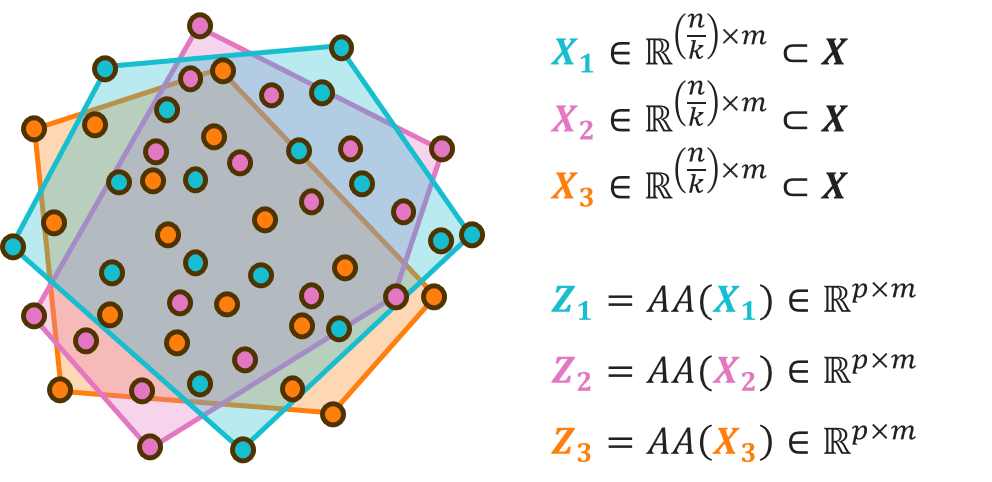
\includegraphics[width=0.6\textwidth]{redRedOutputDataSplit}
    (b)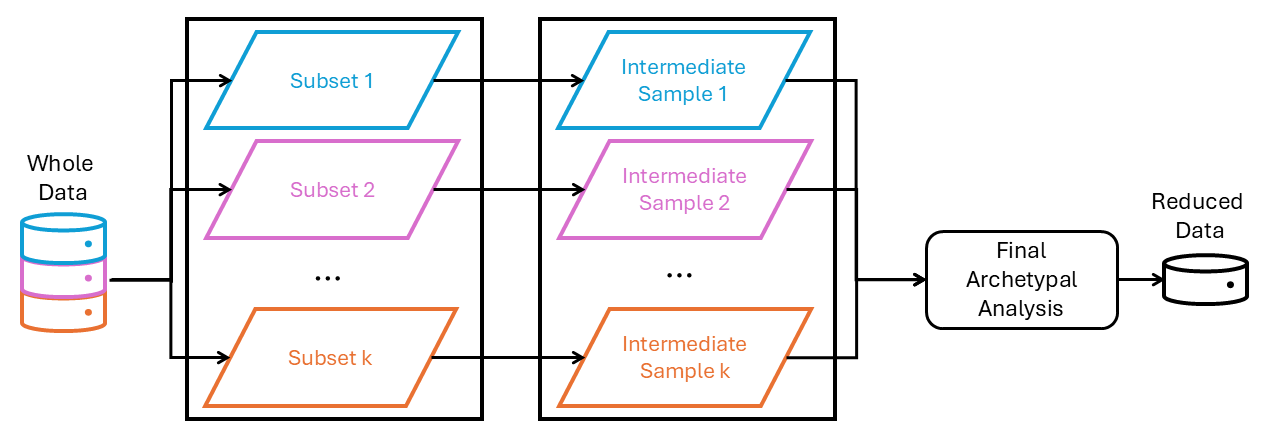
\includegraphics[width=0.95\textwidth]{workflow}
    \caption{Illustration of (a) process of splitting of data into subsets, and (b) workflow of iterative archetypal analysis.\vspace{-5mm}}
    \label{fig:redRedOutputDataSplit}
\end{figure}

\begin{algorithm}
\caption{Pseudocode of iterative archetypal analysis algorithm.}
\label{alg:redRedIAA}
\begin{flushleft}
    \textbf{Input}: \\
    \hspace*{\algorithmicindent} $\mathbf{X} \in \mathbb{R}^{n \times m}:$ Original dataset \\
    \hspace*{\algorithmicindent} $k:$ Number of subsets \\
    \hspace*{\algorithmicindent} $p_1:$ Number of archetypes for initial round of AA (intermediate samples) \\
    \hspace*{\algorithmicindent} $p_2:$ Number of archetypes for final round of AA (output archetypes) \\
    \textbf{Output}: \\
    \hspace*{\algorithmicindent} $\mathbf{Z}_{\mathrm{final}} \in \mathbb{R}^{p_2 \times m}:$ Final archetypes
\end{flushleft}
\begin{algorithmic}[1]
    \Procedure{iterAA}{$\mathbf{X}, k, p_1, p_2$}
        \State Divide $\mathbf{X}$ into $k$ subsets: $\{\mathbf{X}_1, \mathbf{X}_2, \ldots, \mathbf{X}_k\}$
        \State $\mathbf{Z} \gets \emptyset$
        \For{$i = 1$ to $k$}
            \State Apply archetypal analysis on $\mathbf{X}_i$, return $p_1$ archetypes
            \State Obtain intermediate samples $\mathbf{Z}_i \in \mathbb{R}^{p_1 \times m}$
        \EndFor
        \State Combine all intermediate samples: $\mathbf{X}_{\mathrm{subset}} = [\mathbf{Z}_1; \mathbf{Z}_2; \ldots; \mathbf{Z}_k]$
        \State Apply archetypal analysis on $\mathbf{X}_{\mathrm{subset}}$, return $p_2$ archetypes
        \State Obtain final archetypes $\mathbf{Z}_{\mathrm{final}}$
        \State \textbf{return} $\mathbf{Z}_{\mathrm{final}}$
    \EndProcedure
\end{algorithmic}
\end{algorithm}

\subsection{Computational complexity and validity conditions of IAA}

The principal contribution of IAA lies in the way outputs from successive rounds of AA are connected into a unified workflow. One practical advantage of the design is that any AA algorithm capable of returning the archetypes and reconstruction coefficient matrices can serve as the underlying solver, so the exact computational scaling of IAA inherits from the chosen implementation. Execution time is minimised by distributing as many small subsets as possible across all available processor cores. The user needs only to specify the number of intermediate archetypes from the first round and the desired number of final archetypes; parallelisation of the first round reduces the input size for the subsequent round. The overall runtime is bounded by whichever round operates on the larger combination of input and output sizes, which is typically the final round. Although additional rounds of iteration are possible, reconstruction error accumulates with each pass, so more than two iterations are not recommended in practice.

\paragraph{Computational scaling}
Consider a dataset $X \in \mathbb{R}^{N \times d}$ comprising $N$ samples in $d$ dimensions. Alternating minimisation in standard AA involves quadratic programmes with coefficient matrices of size $N \times p_2$ and $p_2 \times N$, so the dominant cost grows no slower than quadratically in $N$.

Under the IAA scheme, $X$ is divided into $k$ roughly equal subsets of size $N/k$, each processed independently to yield $p_1$ intermediate archetypes. These $k p_1$ intermediate samples are then assembled and passed to a single final AA step. The total wall-clock time is therefore
\begin{equation} \label{eq:IAAexeTime}
T_{IAA}(n, m, k, p_1, p_2) = k \times T\left( AA\left( \frac{n}{k}, m, p_1 \right) \right) + T\left( AA\left( p_1 \times k, m, p_2 \right) \right)
\end{equation}
where $T(AA)$ = execution time of AA, $n$ = number of samples, $m$ = number of features, $k$ = number of subsets, $p_1$ = number of archetypes for initial round of AA (intermediate samples), $p_2$ = number of archetypes for final round of AA (output archetypes), and $AA(n, m, p)$ = AA on dataset with $n$ samples and $m$ features, returning $p$ archetypes. When $p_1 \ll N$ and $k \ll N$, this decomposition substantially reduces the quadratic dependence on $N$ relative to applying AA directly to the full dataset.

\paragraph{Assumptions and limitations}
IAA rests on the premise that the convex hull of the complete dataset is adequately captured by the union of convex hulls computed from its constituent subsets. Optimal performance is achieved when the data contain a high degree of structural redundancy and when configurations that lie on or near the extremes of the distribution appear in each subset with reasonable frequency. The method is less reliable for strongly multimodal data, because infrequent but structurally significant modes may not be represented in every subset and can consequently be lost among the intermediate archetypes. When redundancy is low or sampling is already near-uniform, the computational benefit of partitioning may be modest. A further consideration is that an overly small choice of $p_1$ introduces information loss that cannot be recovered in subsequent iterations, since errors compound across rounds. Consequently, no more than two iterations of IAA are advisable in practice.


\subsection{Performance Evaluation} \label{sec:redRedOutputEvaluation}

The performance of IAA was assessed using two synthetic 2D datasets with circular and square distributions, benchmarked against a reference implementation of robust AA~\cite{Chen2014robustAA} with parameters \texttt{Z0}=None, \texttt{returnAB}=True, \texttt{robust}=False, \texttt{tolerance}=0.001, \texttt{computeXtX}=False, \texttt{stepFISTA}=3, \texttt{stepsAS}=50, \texttt{randominit}=False and \texttt{numThreads}=-1. Fig.~\ref{fig:redRedOutput} shows that the archetype locations returned by IAA are in close agreement with those from the reference method. Table~\ref{tab:redRed2DdataEval} confirms that IAA achieves comparable explained variance at shorter execution times, with the runtime decreasing monotonically as the number of subsets increases, for fixed archetype count and dataset dimensionality.
\begin{figure}[t] \centering
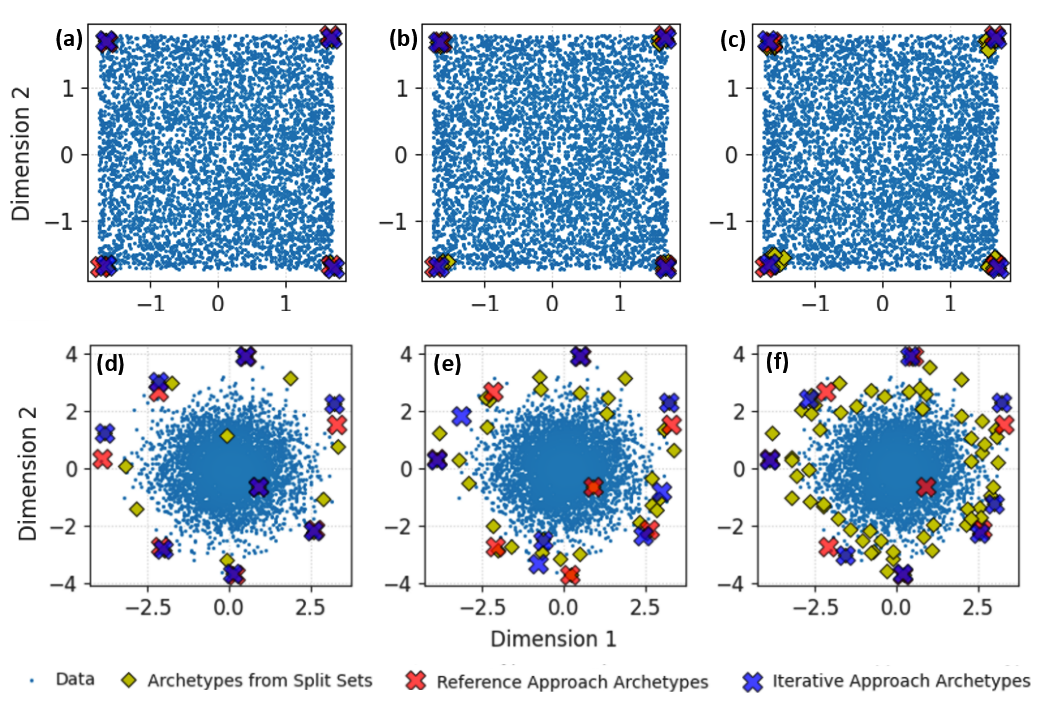
\includegraphics[width=\textwidth]{redRedOutput}
\caption{Distribution of the samples, archetypes obtained from subsets, and final archetypes obtained from reference archetypal analysis and iterative archetypal analysis with 2, 4, and 8 subsets for 2D square dataset (a,b,c), and 2D circular dataset (d,e,f), respectively.\vspace{-5mm}}
\label{fig:redRedOutput}
\end{figure}

\begin{table}[t]
\caption{Comparison between the outputs of reference archetypal analysis and iterative archetypal analysis applied to 2D datasets with 5000 samples. The number of archetypes used for the square and circular datasets are 4 and 8, respectively. The execution times are averaged over 30 runs.}
\centering
\small
\begin{tabular}[width=\textwidth]{l|cc|ccc}
\hline
Dataset & \multicolumn{2}{c|}{RAA} & \multicolumn{3}{c}{IAA}            \\
         & Execution & Explained    & Number of & Execution & Explained \\
         & time (s)  & variance     & subsets   & time (s)  & variance  \\
\hline
Square   & 4.2       & 100.0        & 2         & 0.7       & 100.0     \\
         &           &              & 4         & 0.5       & 100.0     \\
         &           &              & 8         & 0.3       & 100.0     \\
Circular & 6.2       & 100.0        & 2         & 2.2       &  99.9     \\
         &           &              & 4         & 0.6       &  99.6     \\
         &           &              & 8         & 0.4       &  99.9     \\
\hline
\end{tabular}
\label{tab:redRed2DdataEval}
\end{table}

To evaluate the method on real MD simulation trajectories, pairwise conformation similarity is assessed using three complementary representations: three-dimensional Cartesian coordinates ($\mathbb{R}^{i \times 3}$, where $i$ is the number of atoms), average bond length distributions (vectors of length $i$), and the radial distribution function (RDF), which quantifies the probability of finding an atom at a given distance from a reference atom~\cite{Liu2018NPRDF} (vectors of length $j$, where $j$ is the number of distribution points). Coordinate similarity is quantified by the root mean square error (RMSE), which suppresses the influence of large deviations and preserves the original units. Similarity between average bond length distributions is measured by mutual information~\cite{Kinney2014MI}, computed using the \texttt{mutual\_info\_regression} function from the \texttt{scikit-learn} package~\cite{Pedregosa2011sklearn}.

The RDF is computed using the \texttt{rdfpy} package~\cite{Yildirim2021rdfpy}, with a bin width $d_\mathrm{RDF}$ given by Eqn.~\ref{eq:dataCollectOutputRDFint}, and a fixed number of distribution points ($n_\mathrm{points}$=1000) chosen to balance computational cost against statistical power. RDF similarity is evaluated through a suite of two-sample statistical tests that examine the null hypothesis that two RDFs are drawn from the same distribution, i.e., that the corresponding conformations are structurally identical. The tests employed are the two-sample Kolmogorov-Smirnov test~\cite{Conover1965KStest}, the two-sample Cram\'er-von Mises test~\cite{Anderson1962CMtest}, and the two-sample Anderson-Darling test~\cite{Scholz2012ADtest}, all implemented via the \texttt{SciPy} package. Each test is distribution-free when both empirical distributions are continuous and contain no tied values. Divergence-based similarity measures are also employed, including the Wasserstein distance~\cite{Kantorovich1960KantorovichDist}, Hellinger distance~\cite{Beran1977HellingerDist}, Kullback-Leibler divergence~\cite{Kullback1951KLdiv}, and Jensen-Shannon divergence~\cite{Fuglede2004JSdiv}.
\begin{equation} \label{eq:dataCollectOutputRDFint}
d_\mathrm{RDF} = r * M_\mathrm{cutoff} / n_\mathrm{points}
\end{equation}
where $d_\mathrm{RDF}$ = RDF interval size, $r$ = nanoparticle radius, $M_\mathrm{cutoff}$ = radius cutoff multiplier, and $n_\mathrm{points}$ = number of RDF distribution points.

For each pair of nanoparticle conformations, all 10 tests are applied to determine whether one member of the pair is redundant. Each test requires a threshold, which is determined empirically by identifying the cutoff at which successive conformations become visually distinguishable (see Supporting Information, Section S2). This domain-driven approach has limited scalability, which further motivates the use of IAA.


\section{Results}
\label{sec:results}

\subsection{Determination of the Optimal Number of Archetypes}
\label{sec:optNumArch}

\subsubsection{Dataset Overview}
\label{sec:dataset}

The IAA implementation is publicly available on GitHub~\cite{SuppInfo}, together with documentation and links to all public datasets used in this study. The datasets are structurally diverse, encompassing ordered crystalline, disordered non-crystalline, and polycrystalline (including twinned) nanoparticle configurations. Details of the data generation protocol are given in Reference~\cite{Sun2018PtMD}, with full dataset descriptions provided in Supporting Information (Table S1) and the repository~\cite{SuppInfo}. All IAA parameters used in this study are listed in Supporting Information, Table S2, and the repository~\cite{SuppInfo}.

\subsubsection{Elbow-Based Archetype Selection}
\label{sec:elbowSelection}

The elbow criterion is a widely used heuristic~\cite{Fernandez2015clustAA} for selecting an appropriate number of archetypes. As shown in Fig.~\ref{fig:allNPs_expVar}(a,b,c), this criterion suggests 100, 200, and 200 archetypes for the mono-, bi-, and trimetallic datasets, respectively. The corresponding simplex plots in Fig.~\ref{fig:allNPs_expVar}(d,e,f) display the distribution of samples projected onto the simplex defined by the elbow-selected archetypes. However, given the high dimensionality of these datasets, the resulting features-to-samples ratio is large enough to risk overfitting during ML model training, whereby the model learns noise rather than the underlying structure and generalises poorly to unseen data. A larger number of archetypes is therefore required.
\begin{figure}[t] \centering
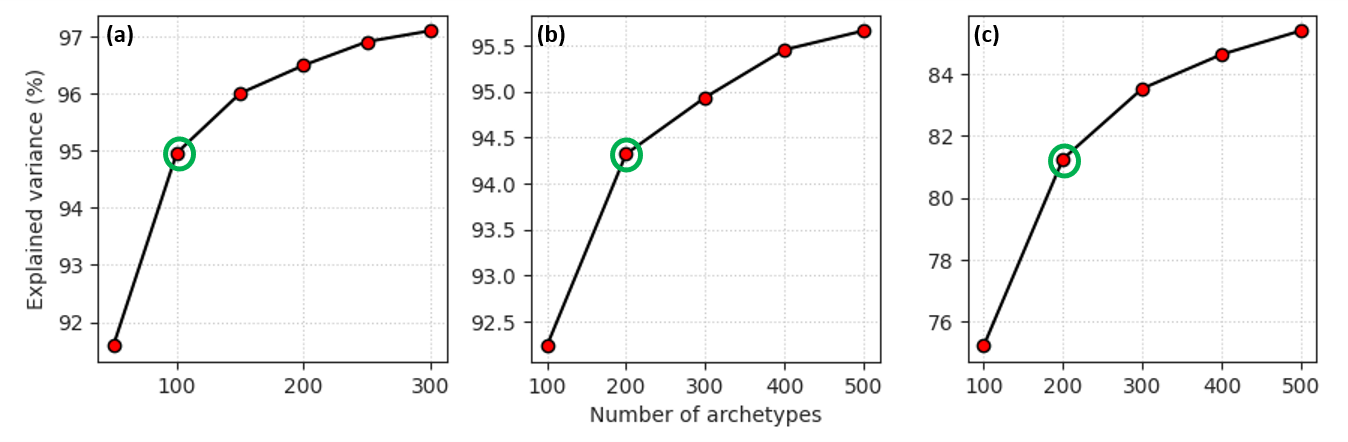
\includegraphics[width=\textwidth]{allNPs_expVar}
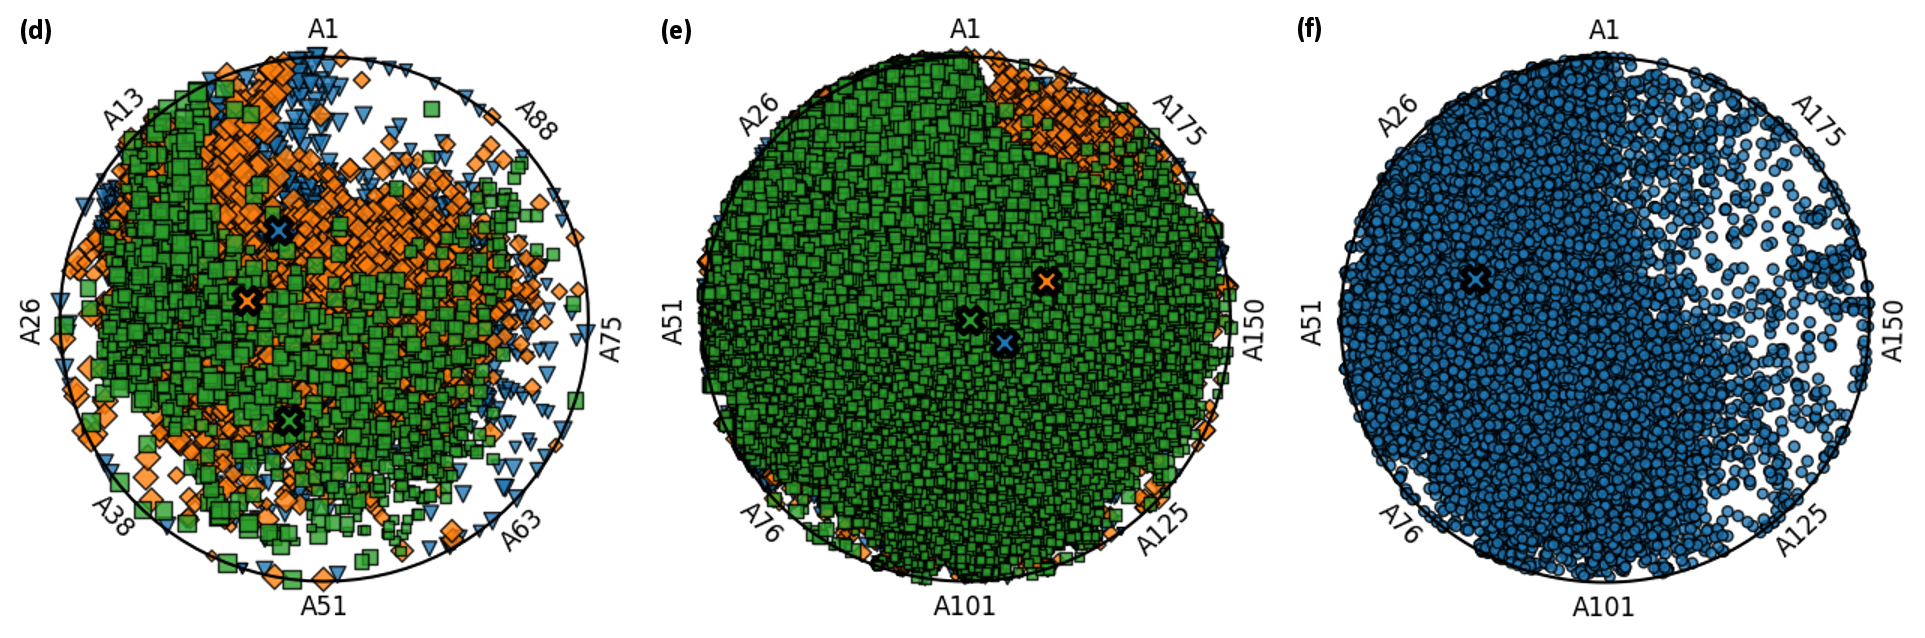
\includegraphics[width=\textwidth]{allNPs_markPrototype_simplex_elbowArchs}
\caption{Elbow plots for the selection of number of archetypes for (a) monometallic, (b) bimetallic, (c) trimetallic nanoparticle datasets. The elbows are highlighted by green circles; simplex plots of the samples for (d) the monometallic Au (blue), Pd (orange), and Pt (green) nanoparticle datasets with 100 archetypes, (e) the bimetallic AuPd (blue), AuPt (orange), and PdPt (green) nanoparticle datasets with 200 archetypes, and (f) the trimetallic AuPdPt (blue) nanoparticle dataset with 200 archetypes. The crosses indicate the hypothetical prototypes with averaged feature values of the samples with identical elemental combinations. Points are sized relative to the average diameters of the nanoparticles.}
\label{fig:allNPs_expVar}
\end{figure}

\subsubsection{Redundancy in Large Archetype Set}
\label{sec:largeSetRedundancy}

Extracting a large number of archetypes (here, 5000 for demonstration) inevitably introduces redundant archetypes that contribute negligibly to the reconstruction of any sample. This is evident in the simplex plots of Fig.~\ref{fig:allNPs_markPrototype_simplex_maxArchs}, which show extensive unpopulated regions near the vertices. In these plots, the contribution of a given archetype to a sample is inversely related to the distance of that sample from the corresponding vertex\footnote{Note that vertices are no longer obvious when a simplex has many vertices.}~\cite{Fernandez2015clustAA}. The absence of samples at or near a vertex indicates that the corresponding archetype either does not exist or has no close match among the original configurations. Furthermore, sparsely populated regions near higher-indexed archetypes suggest that these represent configurations never observed in the simulations. A principled balance between coverage and parsimony is therefore necessary.
\begin{figure}[t] \centering
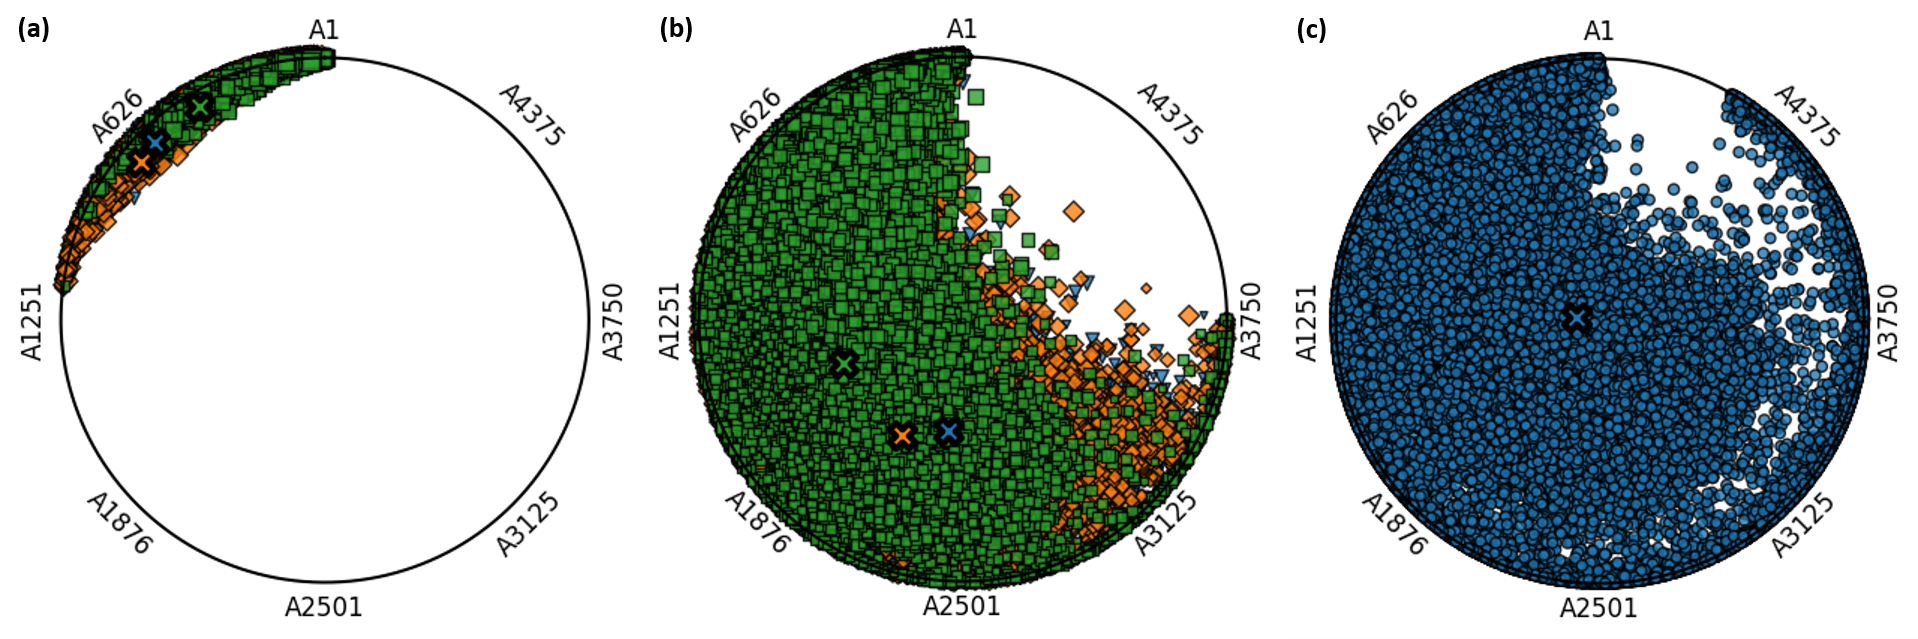
\includegraphics[width=\textwidth]{allNPs_markPrototype_simplex_maxArchs}
\caption{Simplex plots of the samples for (a) the monometallic Au (blue), Pd (orange), and Pt (green), (b) the bimetallic AuPd (blue), AuPt (orange), and PdPt (green), and (c) the trimetallic AuPdPt (blue) nanoparticle datasets with 5000 archetypes. The crosses indicate the hypothetical prototypes with averaged feature values and the same elemental combinations. Points are sized relative to the average diameters of the nanoparticles.\vspace{-5mm}}
\label{fig:allNPs_markPrototype_simplex_maxArchs}
\end{figure}

\subsubsection{Quantitative Criteria for Archetype Optimisation}
\label{sec:quantCriteria}

Simplex visualisation can be complemented by quantitative criteria derived from reconstruction quality and the degree to which each archetype is utilised. One common approach is to set a target explained variance threshold; however, this introduces its own difficulties. For the monometallic dataset, 100 archetypes suffices to reach 95\% explained variance (though at the risk of overfitting), whereas 5000 archetypes still yields only 91\% explained variance for the trimetallic dataset (risking the inclusion of redundant archetypes). Given that preserving information takes precedence over minimising dataset size, including more archetypes is the safer choice when in doubt. The ideal number of archetypes is the smallest value for which every archetype can be matched to a sample present in the original dataset. In this work, the explained variance serves as a lower bound on reconstruction fidelity, and is used in conjunction with the distribution of archetypal contributions encoded in the coefficient matrix $A$. Redundant archetypes are characterised by consistently near-zero weights across all samples; a practical indicator of this is the sparsity or entropy of the column-wise distributions of $A$, where archetypes with negligible average contributions or vanishingly small support signal over-parameterisation. In addition, the minimum distance from each archetype to its nearest original sample can flag archetypes that do not correspond to any physically realised configuration. Together, these metrics provide objective criteria for reducing $p_2$ without relying solely on visual assessment.

\subsubsection{Iterative Optimisation}
\label{sec:iterOptim}

The appropriate number of archetypes is found by progressively reducing from 5000 (a value known to introduce redundancy) until the vertices of the simplex plots are fully or very nearly occupied by samples present in the original dataset. The pattern of vacant regions in Fig.~\ref{fig:allNPs_markPrototype_simplex_maxArchs} provides guidance on how far to reduce, but the optimal configuration depends on the specific archetype count chosen, so several iterations are typically needed to arrive at a solution in which all vertices are occupied. Although this process involves some degree of user judgement, it is designed to accommodate different research objectives and available computational resources. A sequence of simplex plots illustrating this process is provided in Supporting Information (Section S6) and the repository~\cite{SuppInfo}. Comparing these plots with Fig.~\ref{fig:allNPs_markPrototype_simplex_maxArchs} reveals that the prototype position generally migrates toward the centre of the simplex as redundant archetypes are removed, since their presence distorts the distribution of archetypal contributions and shifts the prototype away from the centre. However, a centrally located prototype is a necessary but not sufficient condition for the absence of redundancy (see Supporting Information, Fig. S8, and the repository~\cite{SuppInfo}): a displaced prototype reliably signals redundancy, but a centred prototype does not guarantee its absence.

The final archetype counts are 250, 1800, and 3000 for the mono-, bi-, and trimetallic datasets, respectively, as reflected in Fig.~\ref{fig:allNPs_markPrototype_simplex_bestArchs}, which shows even sample distributions across the simplex and vertices that are fully or nearly occupied by configurations drawn from the original data. To ensure a favourable ratio of samples to features during subsequent ML model training, dimensionality reduction in the feature space (removal of highly correlated features and selection of domain-relevant features) should be performed after AA. Summary statistics of the reduced datasets are given in Table~\ref{tab:redRedOutcomeReducedData}. Representative radar plots illustrating the archetypal contributions for randomly selected samples from both dense and sparse simplex regions are provided in Supporting Information, Figs. S10, S11, and S12, and the repository~\cite{SuppInfo}. Depending on research objectives and available resources, alternative values of $n$ could be selected.
\begin{figure}[t] \centering
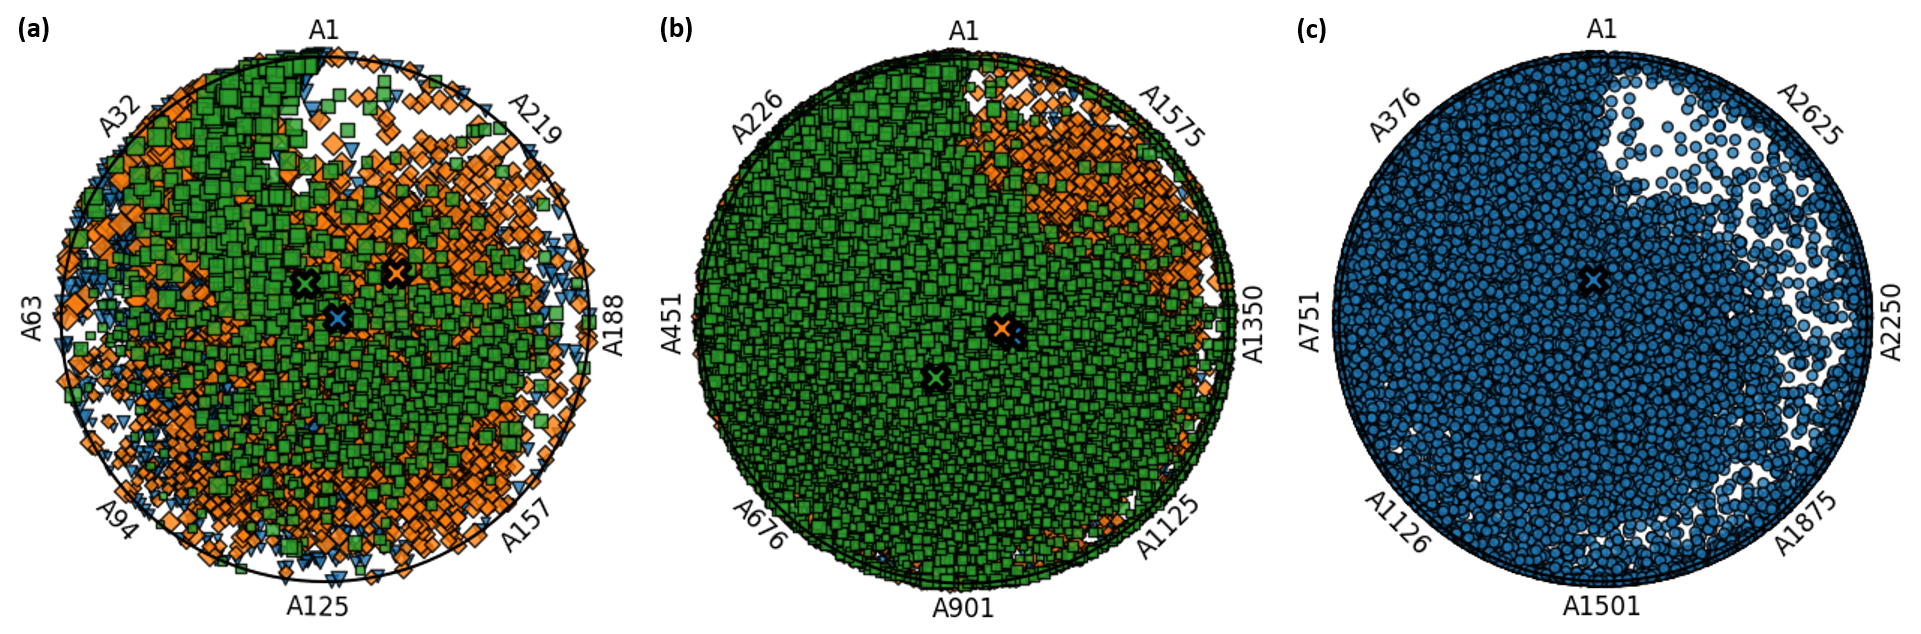
\includegraphics[width=\textwidth]{allNPs_markPrototype_simplex_bestArchs}
\caption{Simplex plots of the samples for (a) the monometallic Au (blue), Pd (orange), and Pt (green) nanoparticle datasets with 250 archetypes, (b) the bimetallic AuPd (blue), AuPt (orange), and PdPt (green) nanoparticle datasets with 1800 archetypes, and (c) the trimetallic AuPdPt (blue) nanoparticle dataset with 3000 archetypes. Prototypes indicated by crosses, and point size corresponds to nanoparticle diameters. \vspace{-5mm}}
\label{fig:allNPs_markPrototype_simplex_bestArchs}
\end{figure}

\begin{table}[t]
\caption{Descriptions of the number of samples ($n$) of the original and reduced monometallic, bimetallic, and trimetallic nanoparticle datasets.}
\centering
\small
\begin{tabular}[width=\textwidth]{l|cccc}
\hline
Dataset      & Original $n$ & Final $n$ & Reduction percentage ($\%$) & Explained variance \\
\hline
Monometallic &         9300 &       250 &                        97.3 &               95.0 \\
Bimetallic   &       917373 &      1800 &                        99.8 &               96.4 \\
Trimetallic  &        48136 &      3000 &                        93.8 &               90.3 \\
\hline
\end{tabular}
\label{tab:redRedOutcomeReducedData}
\end{table}


\subsection{Validation Case: Total and Formation Energy Regression}
\label{sec:MNPregEtotEform}

To confirm that the IAA-reduced datasets preserve physically meaningful structure-property relationships, we examine the predictive performance of models trained on the reduced monometallic nanoparticle dataset for both total and formation energy, and compare these against models trained on the complete training set. Formation energy is selected as a particularly demanding test case because of its strong sensitivity to atomic configuration, meaning that even subtle structural differences can alter the target value substantially. Satisfactory prediction of this quantity provides evidence that the reduced dataset retains the structural information governing the system. All code and data for this section are available in a dedicated repository~\cite{MNPERegRepo}.

\subsubsection{Feature Selection}
\label{sec:featSelection}

Feature selection was conducted ahead of model training to limit redundancy and constrain model complexity. Any feature with zero variance was excluded, and when two features exceeded a Pearson correlation of 0.8, the second of the pair was retained. Features were additionally ranked by experimental interpretability where this was applicable. The selected feature set formed the input to all subsequent supervised regression models. Correlation matrices for the retained features are shown in Figure~\ref{fig:MNPCorrHeatmap}.

\begin{figure}[htbp]
    \begin{subfigure}{\textwidth}
        \centering
        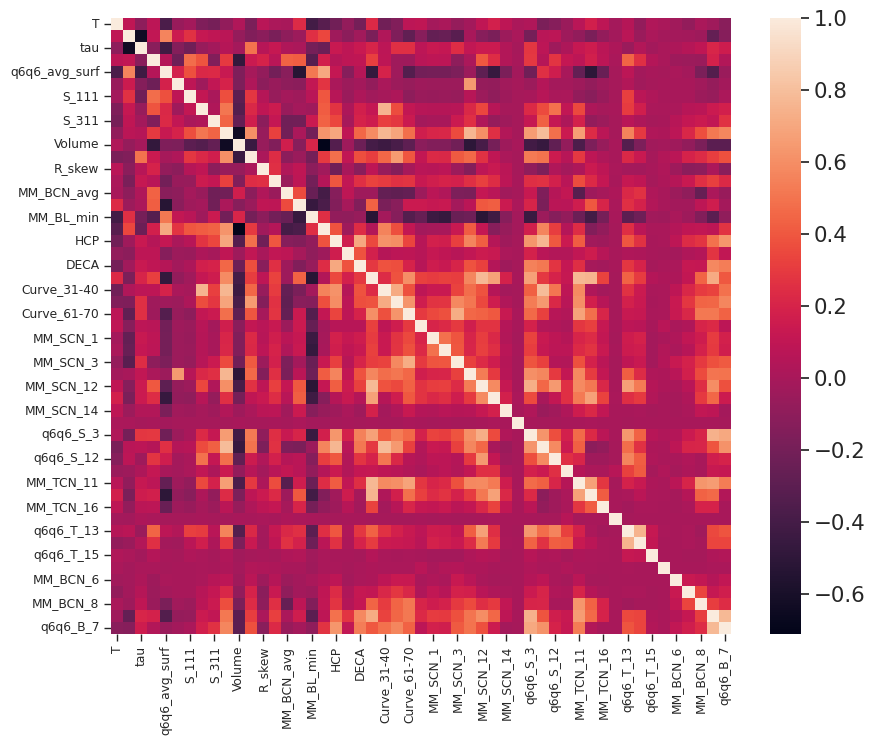
\includegraphics[width=0.98\textwidth]{MNPENoC80CorrHeatmap}
        \caption{} \label{fig:MNPNoC80CorrHeatmap}
    \end{subfigure}
    \begin{subfigure}{\textwidth}
        \centering
        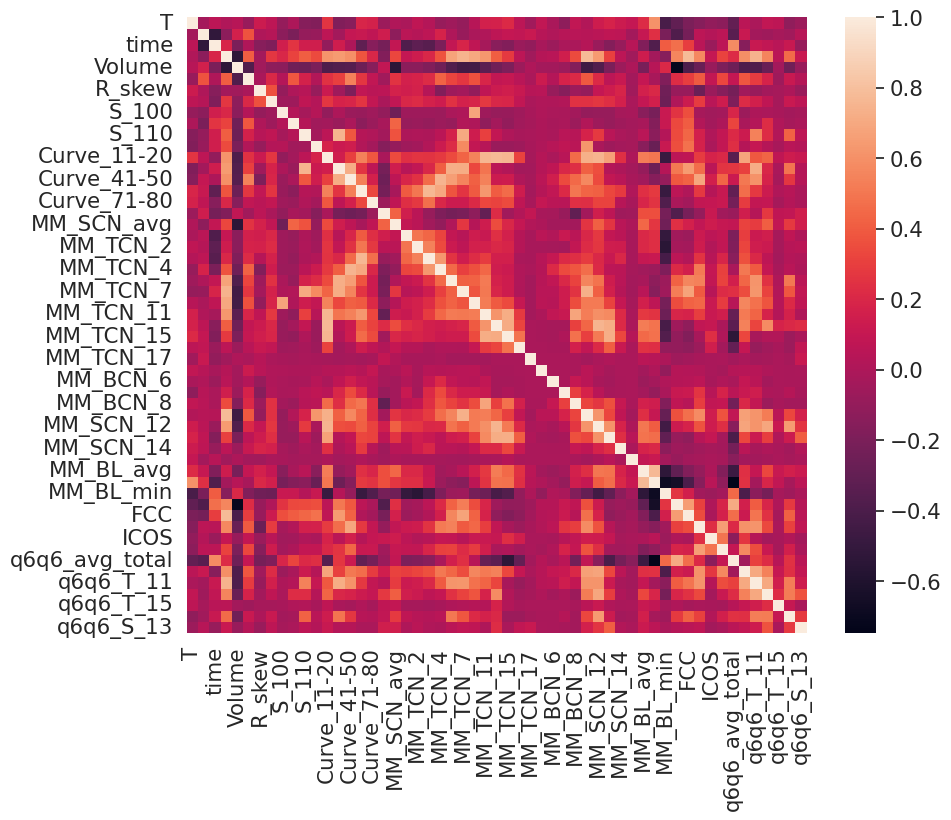
\includegraphics[width=0.63\textwidth]{redMNPENoC80CorrHeatmap}
        \caption{} \label{fig:redMNPNoC80CorrHeatmap}
    \end{subfigure}
    \caption{Correlation matrices of features from the monometallic nanoparticles data set, with (a) all training samples and (b) most archetypal samples.}
    \label{fig:MNPCorrHeatmap}
\end{figure}

\subsubsection{Model Training and Hyperparameter Optimisation}
\label{sec:modelTrain}

An 80:20 split was used to divide the data into training and testing sets. A random forest regressor was selected for its robustness to nonlinear feature relationships and its minimal distributional assumptions. Hyperparameter tuning was carried out by random search over 1000 parameter combinations using 5-fold cross-validation, with the coefficient of determination ($R^2$) as the scoring metric. The explored parameter ranges and the resulting optimal hyperparameters are listed in Table~\ref{tab:RFoptimisedHP}. All additional parameters required to reproduce the reported results are: \textit{min\_weight\_fraction\_leaf}=0.0, \textit{min\_impurity\_decrease}=0.0, \textit{bootstrap}=True, \textit{oob\_score}=False, \textit{random\_state}=42, \textit{warm\_start}=False, \textit{ccp\_alpha}=0.0, \textit{max\_samples}=None, \textit{monotonic\_cst}=None.

\begin{table}[hp!]
    \caption{Hyperparameters optimised \textit{via} random search using random forest regressors over 1000 combinations, fitted to whole training set and most archetypal samples. $E_{Total}$ and $E_{Formation}$ represent total and formation energies, respectively. `se', `ae', and `fm' are abbreviations for `squared\_error', `absolute\_error', and `friedman\_mse', respectively.}
    \centering
    \small
    \begin{tabular}{c|c|cc|cc}
        \hline
        Hyperparameter               &   Range explored &                                        \multicolumn{4}{c}{Optimal value} \\
        \cline{3-6}
                                     &                  & \multicolumn{2}{c}{All samples} & \multicolumn{2}{c}{Archetypal samples} \\
        \cline{3-6}
                                     &                  &  $E_{Total}$ &  $E_{Formation}$ &     $E_{Total}$ &      $E_{Formation}$ \\
        \hline
        \texttt{n\_estimators}       &            3-100 &           82 &              30  &              78 &                   21 \\
        \texttt{criterion}           & `se', `ae', `fm' &         `se' &             `fm' &            `se' &                 `fm' \\
        \texttt{max\_depth}          &             1-10 &            7 &                8 &               6 &                    8 \\
        \texttt{max\_features}       &          0.1-1.0 &        0.887 &            0.823 &           0.799 &                0.816 \\
        \texttt{max\_leaf\_nodes}    &            5-100 &           97 &               98 &              62 &                   72 \\
        \texttt{min\_samples\_leaf}  &             1-10 &            3 &                6 &               2 &                    1 \\
        \texttt{min\_samples\_split} &             2-20 &            6 &                4 &               3 &                    2 \\
        \hline
    \end{tabular}
    \label{tab:RFoptimisedHP}
\end{table}

\subsubsection{Model Performance}
\label{sec:modelPerformance}

Learning curves and evaluation results for the optimised regressors are presented in Figure~\ref{fig:RFRresultsEtotform}. Models trained on the archetypal samples achieved strong predictive performance for both energy targets, with slight underfitting and overfitting observed for formation energy. The somewhat reduced performance on formation energy is consistent with its greater sensitivity to fine-grained structural variation, making it a more exacting test of dataset quality.

For total energy, the model trained on archetypal samples achieved $R^2$ scores of 0.993 (training), $0.969 \pm 0.011$ (cross-validation), and 0.972 (testing). These are comparable to the scores obtained when all training samples are used: 0.998 (training), $0.995 \pm 0.001$ (cross-validation), and 0.994 (testing). For formation energy, the archetypal-sample model achieved $R^2$ scores of 0.986 (training), $0.866 \pm 0.072$ (cross-validation), and 0.931 (testing), compared with 0.993 (training), $0.990 \pm 0.001$ (cross-validation), and 0.991 (testing) when all training samples are used.

\begin{figure}[htbp]
    \centering
        \begin{subfigure}{0.46\textwidth}
        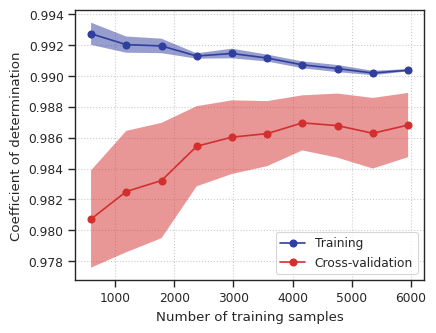
\includegraphics[width=\textwidth]{MNPELearnCurveRFR_Etot_minmax}
        \caption{} \label{fig:MNPELearnCurveRFR_Etot_minmax}
    \end{subfigure}
    \begin{subfigure}{0.47\textwidth}
        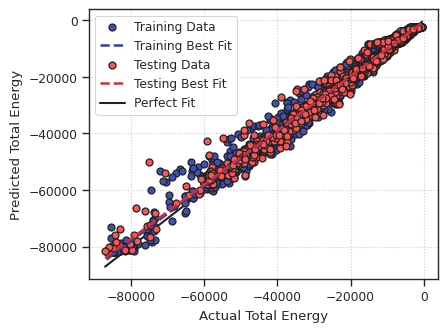
\includegraphics[width=\textwidth]{MNPR2AllRFR_Etot_minmax}
        \caption{} \label{fig:MNPER2AllRFR_Etot_minmax}
    \end{subfigure}
    \begin{subfigure}{0.47\textwidth}
        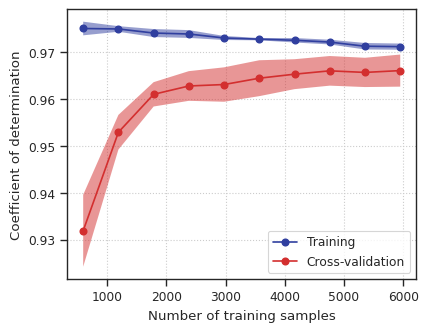
\includegraphics[width=\textwidth]{MNPELearnCurveRFR_Eform_minmax}
        \caption{} \label{fig:MNPELearnCurveRFR_Eform_minmax}
    \end{subfigure}
    \begin{subfigure}{0.47\textwidth}
        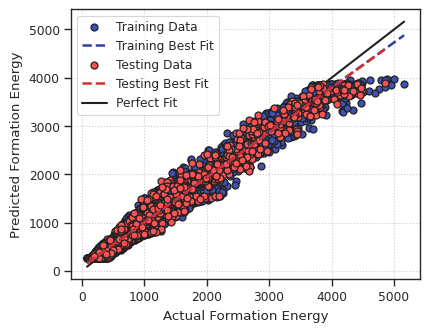
\includegraphics[width=\textwidth]{MNPR2AllRFR_Eform_minmax}
        \caption{} \label{fig:MNPER2AllRFR_Eform_minmax}
    \end{subfigure}
    \begin{subfigure}{0.45\textwidth}
        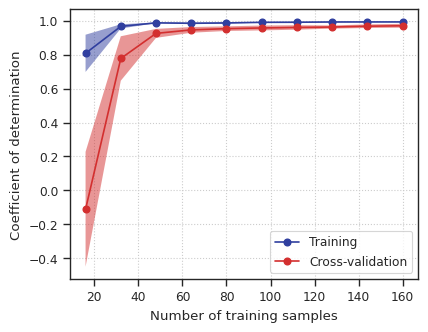
\includegraphics[width=\textwidth]{MNPELearnCurveRFR_red_Etot_minmax}
        \caption{} \label{fig:MNPELearnCurveRFR_red_Etot_minmax}
    \end{subfigure}
    \begin{subfigure}{0.47\textwidth}
        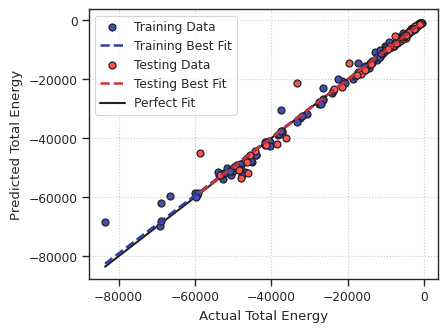
\includegraphics[width=\textwidth]{MNPR2AllRFR_red_Etot_minmax}
        \caption{} \label{fig:MNPR2AllRFR_red_Etot_minmax}
    \end{subfigure}
    \begin{subfigure}{0.47\textwidth}
        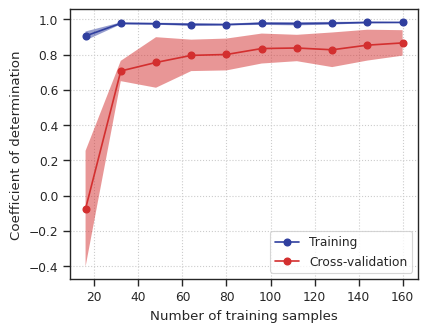
\includegraphics[width=\textwidth]{MNPELearnCurveRFR_red_Eform_minmax}
        \caption{} \label{fig:MNPELearnCurveRFR_red_Eform_minmax}
    \end{subfigure}
    \begin{subfigure}{0.47\textwidth}
        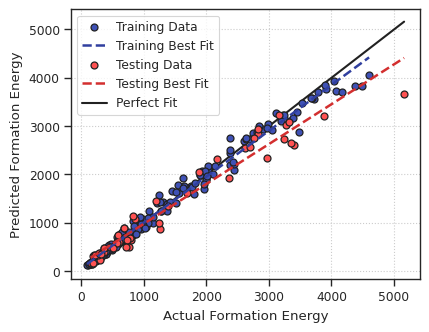
\includegraphics[width=\textwidth]{MNPR2AllRFR_red_Eform_minmax}
        \caption{} \label{fig:MNPR2AllRFR_red_Eform_minmax}
    \end{subfigure}
    \caption{Results of the optimised random forest regressors fitted to (a-d) all training samples and (e-h) most archetypal samples, predicting the (a-b, e-f) total energy and (c-d, g-h) formation energy of monometallic nanoparticles: (a, c, e, g) learning curves and (b, d, f, h) scatter plots of predictions on training and testing sets.}
    \label{fig:RFRresultsEtotform}
\end{figure}

These results confirm that the IAA-reduced dataset retains the structural information required for accurate energy prediction. The close alignment between training, validation, and testing performance indicates low overfitting and good generalisation, demonstrating that the reduction in dataset size does not compromise predictive quality.

To establish that the observed improvements stem from the IAA sampling strategy rather than from simply working with a smaller dataset, a baseline was constructed using randomly drawn subsets of equal size. The random sampling and model fitting procedures were repeated over 10 independent iterations. For total energy, the average $R^2$ scores were 0.992 (training), $0.961 \pm 0.019$ (validation), and 0.957 (testing). For formation energy, the corresponding averages were 0.981 (training), $0.892 \pm 0.043$ (validation), and 0.895 (testing). In both cases, models trained on IAA-selected samples consistently outperformed those trained on randomly selected samples of equivalent size.

Consistent trends were observed when linear regressors replaced the random forest models, reinforcing the generalisability of these findings across model classes. The corresponding results are reported in Supporting Information, Section S9.

Taken together, these comparisons show that the advantage conferred by IAA arises from the quality of the selected samples rather than the reduction in quantity alone. By preserving broad coverage of the feature space while eliminating redundant configurations, IAA produces datasets that are more informative and better suited for downstream machine learning.

The results confirm that IAA is capable of substantially reducing dataset size while maintaining or even enhancing the predictive performance of models trained on the reduced data.



\section{Discussion}
\label{sec:discussion}

Application of IAA to the metallic nanoparticle datasets produces substantially smaller datasets with reduced redundancy, opening the door to further independent analyses. A direct comparison with the conventional domain-driven approach, which removes redundant samples using pairwise similarity thresholds (see Supporting Information, Table S1, and the repository~\cite{SuppInfo}), illustrates the magnitude of the difference: for the bimetallic dataset, IAA achieved a 99.8\% reduction in sample count, compared with only 67.2\% for the domain-driven method. The practical consequence for model training is dramatic: ML algorithms such as linear regressors (scaling as $O(nm^2+m^3)$) and support vector machines (scaling as $O(n^3)$) can be trained approximately 500 and 125,000,000 times faster, respectively, when using IAA-extracted datasets in place of domain-filtered ones. Although applying more stringent domain-driven thresholds could in principle yield further reductions, doing so risks preferential removal of low-energy configurations, introducing selection bias. IAA avoids this problem entirely by dispensing with user-defined thresholds, thereby minimising the subjective element of the redundancy removal process.

To demonstrate that the IAA-reduced datasets are more informatively sampled than those produced by the domain-driven approach, we draw on concepts from active learning for regression~\cite{Wu2019GSx}. The objective of active learning is to identify the smallest set of labelled samples needed to train an effective ML model~\cite{Tharwat2023AL}. A widely used sampling criterion in active learning is greedy sampling on the inputs (GSx)~\cite{Wu2019GSx}, which selects samples that maximise diversity in the feature space by choosing at each step the point most distant from all previously selected points. Inspired by this framework, we adopt the GSx diversity metric (Eqn.~\ref{eq:GSx}) to compare the feature-space coverage of the domain-driven and IAA-reduced datasets.
\begin{equation} \label{eq:GSx}
    div_{\mathrm{GS}_x} = \frac{1}{N} \sum_i^N \min\limits_{j \neq i} d(R_i, R_j)
\end{equation}
where $d(x, y)$ = distance between instances $x$ and $y$, $R$ = reduced dataset, and $N$ = $|R|$, number of samples in $R$.

A higher value of this metric indicates that samples are more widely separated in feature space, reflecting greater overall diversity. The IAA-reduced dataset achieves a diversity score of $div_{\mathrm{GS}_x} = 2919.8$, more than an order of magnitude larger than the domain-driven reduced dataset ($div_{\mathrm{GS}_x} = 247.2$), underscoring the superiority of IAA for extracting diverse, non-redundant subsets from MD trajectories. This is corroborated by the feature profiles shown in Fig.~\ref{fig:allNPs_maxArchs_compareFeatProfRadarPlots_allFeats}, which span the full extent of the feature space, confirming that the archetypal samples are both diverse and unbiased with respect to coverage. The empty sections in the monometallic profile (Fig.~\ref{fig:allNPs_maxArchs_compareFeatProfRadarPlots_allFeats}(a)) correspond to features with constant values that carry no information for the archetype computation. Because the retained samples are the closest matches to the computed archetypes, examining their feature profiles offers insight into the distinctive characteristics of the non-redundant configurations preserved in the reduced datasets.
\begin{figure}[t] \centering
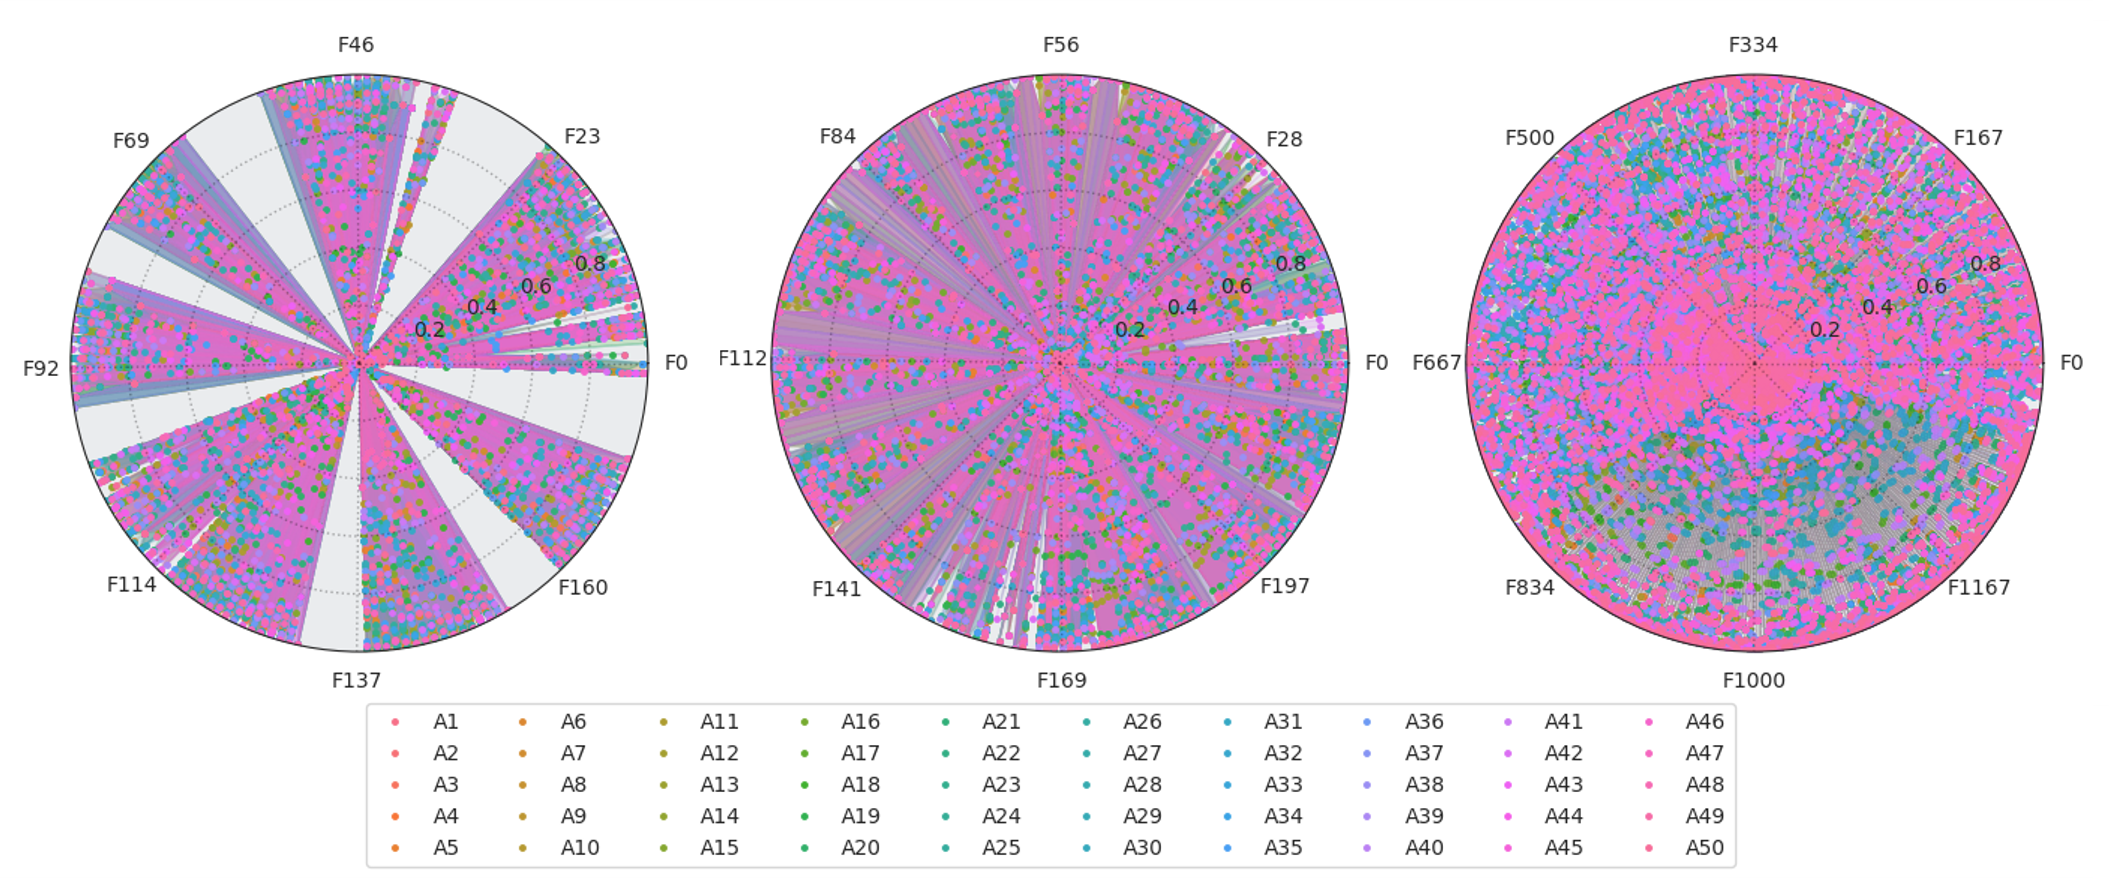
\includegraphics[width=\textwidth]{allNPs_maxArchs_compareFeatProfRadarPlots_allFeats}
\caption{Radar plots of feature profiles for all archetypes of (a) monometallic, (b) bimetallic, and (c) trimetallic nanoparticle datasets (only the first 50 archetypes are included to avoid cluttering). ``A" and ``F" represent archetype and feature, respectively. The empty sections in (a) represent features with constant values that do not contribute to the computation of archetypes.}
\label{fig:allNPs_maxArchs_compareFeatProfRadarPlots_allFeats}
\end{figure}

Several natural extensions of this work suggest themselves. Because the number of intermediate archetypes from the first round can differ from the number of final archetypes, it would be worth exploring different AA algorithms or acceleration strategies at each stage, or even mixing approaches within a single workflow. For instance, computationally expensive methods that preserve more information could be used in early iterations, with lighter-weight methods reserved for later ones. Additional work could also investigate the sensitivity of results to initialisation, or incorporate the \texttt{AA++} initialisation scheme of Mair and Sj{\"o}lund~\cite{Mair2023AA++}, which reduces the likelihood of convergence to poor local minima through a more principled starting strategy.

In the current work, IAA is applied before feature selection to permit fair comparisons, but reversing this order may yield different results and warrants separate investigation. Furthermore, the iterative search for the optimal archetype count currently relies on trial-and-error; convergence could be accelerated using the Newton-Raphson method~\cite{Meza2011NewtonRaphson}. Ultimately, developing a fully automated procedure for selecting the number of archetypes (perhaps by quantifying redundancy in the archetypal space through the sparsity of the simplex plots) would further reduce subjective input and improve the reproducibility of the workflow.


\section{Conclusion}
\label{sec:conclusion}

We have introduced an iterative approach to archetypal analysis and, for the first time, applied it to the extraction of compact, representative sample sets from molecular dynamics trajectories. The performance of iterative archetypal analysis was benchmarked on three structural datasets from MD simulations, in comparison with a reference active set implementation, demonstrating speedups of up to an order of magnitude with negligible reduction in explained variance. The archetypal subsets achieved a 99.8\% reduction in the sample space, far exceeding the 67.2\% reduction obtained by domain-knowledge-based filtering; the consequence for ML model training is a potential speedup of hundreds of thousands of times. This work establishes a pathway to obtaining representative, low-redundancy data subsets from large-scale MD datasets, and provides an entirely unsupervised, data-driven, and reproducible framework for preparing MD simulation data for machine learning.\par



\medskip
\textbf{Supporting Information} \par
Supporting Information is available from the Wiley Online Library or from the author.



\medskip
\textbf{Acknowledgements} \par
Computational resources for this project were supplied by the National Computing Infrastructure (NCI) [grant numbers p00 and q27]. Jonathan Y. C. Ting is grateful for the support from Australian National University via the University Research Scholarship. 



\medskip
\textbf{Declaration of Competing Interest} \par
The authors declare no conflict of interest.



\medskip
\textbf{Data Availability} \par
The software is available at: \url{https://github.com/Jon-Ting/iteraa}, together with details and links to the free datasets used in this study.



\medskip
\bibliographystyle{MSP}
\bibliography{ref}



\begin{figure}
\textbf{Table of Contents}\\
\medskip
  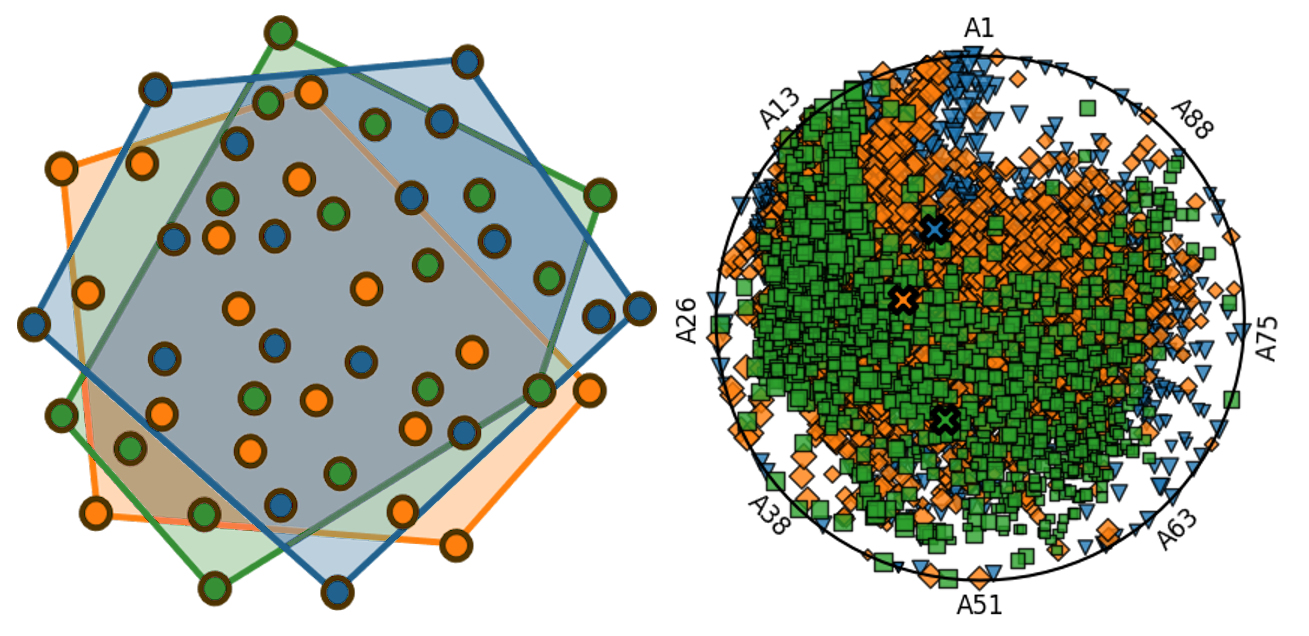
\includegraphics[width=0.75\textwidth]{toc}
  \medskip
  \caption*{Molecular dynamics (MD) is an efficient way of generating data, but many configurations are redundant. Iterative Archetypal Analysis (IAA) is an effective way of isolating non-redundant configurations, minimising the data volume while maximising information.}
\end{figure}


\end{document}
